\documentclass[aspectratio=169]{beamer}

%\includeonlyframes{current}

\usepackage[utf8]{inputenc}
\usepackage[american]{babel}
\usepackage{amsmath,amsthm}
\usepackage{unicode}
\usepackage{array,tabularx}
\usepackage{ifthen}
\usepackage{tikz}
\usetikzlibrary{matrix,decorations,decorations.text,calc,arrows,snakes,shapes,positioning,patterns}
\usepackage{tikzsymbols}

\usepackage{ulem}

\mode<presentation>{%
  \usetheme{ibm}
}

\newcommand{\C}{ℂ}
\newcommand{\R}{ℝ}
\newcommand{\Z}{ℤ}
\newcommand{\N}{ℕ}
\newcommand{\Q}{ℚ}
\newcommand{\F}{\mathbb{F}}
\renewcommand{\P}{\mathbb{P}}
\renewcommand{\O}{\mathcal{O}}
\newcommand{\tildO}{\mathcal{\tilde{O}}}
\newcommand{\poly}{\operatorname{poly}}
\newcommand{\polylog}{\operatorname{polylog}}
\newcommand{\End}{\operatorname{End}}
\newcommand{\Hom}{\operatorname{Hom}}
\newcommand{\Cl}{\operatorname{Cl}}
\newcommand{\GL}{\operatorname{GL}}
\newcommand{\SL}{\operatorname{SL}}
\newcommand{\cyc}[1]{{〈 #1 〉}}
\newcommand{\sm}[2]{\left(\protect\begin{smallmatrix}#1\protect\\#2\protect\end{smallmatrix}\right)}

\renewcommand{\a}{\mathfrak{a}}
\renewcommand{\b}{\mathfrak{b}}
\newcommand{\g}{\mathfrak{g}}
\newcommand{\G}{\mathcal{G}}
\newcommand{\E}{\mathcal{E}}

\title{Isogeny-based Cryptography}
\author{Luca De Feo}
\date[June 19-20, 2024, PQ-TLS summer school]{June 19-20, 2024\\
  PQ-TLS summer school}
\institute{IBM Research Zürich}

\begin{document}

\frame[plain]{\titlepage}

%%

\begin{frame}{Isogenies: What? Why?}
  \large
  \begin{itemize}
    \setlength{\itemsep}{2em}
  \item A descendant of Elliptic Curve Cryptography.
  \item A rich topic, with many cryptographic applications.
  \item A post-quantum generalization of discrete logarithm cryptography\dots
  \item \dots and much more!
  \item A field moving (too) fast!
  \end{itemize}
\end{frame}

%%

\begin{frame}{This course}
  \begin{description}
    \setlength{\itemsep}{2em}
  \item[Today:] Isogeny crypto without isogenies:
    \begin{itemize}
    \item Cryptographic group actions
    \item Something new
    \end{itemize}
  \item[Tomorrow:] The foundations
    \begin{itemize}
    \item Isogenies
    \item Endomorphism rings
    \item Complex and quaternionic multiplication
    \end{itemize}
  \item[Not covered:]
    \begin{itemize}
    \item The SIDH/SIKE attacks
    \item Higher dimensional abelian varieties
    \item Pre-quantum uses of isogenies
    \item A lot of protocols
    \end{itemize}
  \end{description}
\end{frame}

%%

\begin{frame}[plain]
  \begin{beamercolorbox}[sep=0.1px,center,wd=\paperwidth,sep=0.5\paperheight]{palette tertiary}
    \Huge\centering Cryptographic Group Actions
  \end{beamercolorbox}
\end{frame}

%%

\begin{frame}{A cyclic group}
  \Large
  \centering
  \begin{tikzpicture}
    \node at (0,0) {$G = \langle g\rangle$};
    
    \node (g) at (0:4) {$g$};
    \node (g2) at (30:4) {$g^2$};
    \node at (60:4) {$g^3$};
    \node at (-30:4) {$g^n = g^0 = 1$};
    
    \draw (5:4) arc (5:25:4) (35:4) arc (35:55:4) (-25:4) arc (-25:-5:4);
    \draw[dashed] (65:4) arc (65:325:4);
  \end{tikzpicture}
\end{frame}

%%

\begin{frame}{What's needed for key exchange?}
  \begin{columns}
    \begin{column}{0.5\textwidth}
      \centering
      \begin{tikzpicture}
        \begin{uncoverenv}<-3>
          \begin{scope}
            \def\crater{13}
            \def\jumpa{-8}
            \def\diam{2.5cm}

            \uncover<1>{
              \foreach \i in {1,...,\crater} {
                \draw[blue!20!white] (360/\crater*\i : \diam) to[bend right] (360/\crater*\i+360/\crater : \diam);
              }
            }

            \uncover<2->{
              \pgfmathparse{int(\crater/2)}
              \let\last\pgfmathresult
              \foreach \i in {1,...,\last} {
                \pgfmathparse{mod(pow(2,\i-1),\crater)}
                \let\e\pgfmathresult
                \draw[red] (360/\crater*\e : \diam) to[bend left] (360/\crater*\e*2 : \diam);
                \draw[red] (-360/\crater*\e : \diam) to[bend right] (-360/\crater*\e*2 : \diam);
              }
            }

            \uncover<3->{
              \pgfmathparse{int(\crater/2)}
              \let\last\pgfmathresult
              \foreach \i in {1,...,\last} {
                \pgfmathparse{mod(pow(6,\i-1),\crater)}
                \let\e\pgfmathresult
                \draw[blue] (360/\crater*\e : \diam) to[bend right] (360/\crater*\e*6 : \diam);
                \draw[blue] (-360/\crater*\e : \diam) to[bend left] (-360/\crater*\e*6 : \diam);
              }
            }
            
            \pgfmathparse{\crater-1}
            \let\last\pgfmathresult
            \foreach \i in {0,...,\last} {
              \draw[fill] (360/\crater*\i: \diam) circle (2pt) +(360/\crater*\i: 0.5) node{$g^{\i}$};
            }
          \end{scope}
        \end{uncoverenv}
        
        \begin{uncoverenv}<4->
          \begin{scope}
            \def\crater{12}
            \def\jumpa{5}
            \def\diam{2.5cm}

            \foreach \i in {1,...,\crater} {
              \draw[red] (360/\crater*\i : \diam) to[bend right] (360/\crater*\i+360/\crater : \diam);
              \draw[blue] (360/\crater*\i : \diam) to[bend right=10] (360/\crater*\i+\jumpa*360/\crater : \diam);
            }

            \foreach \i in {1,...,\crater} {
              \pgfmathparse{int(mod(pow(2,\i-1),\crater+1))}
              \let\e\pgfmathresult
              \draw[fill] (360/\crater*\i: \diam) circle (2pt) +(360/\crater*\i: 0.5) node{$g^{\e}$};
            }
          \end{scope}
        \end{uncoverenv}
      \end{tikzpicture}
    \end{column}
    \begin{column}{0.4\textwidth}
      The axioms of a dlog group:
      \begin{itemize}
      \item[\sout{prod:}] \sout{$g^ag^b = g^{a+b}$,}
      \item[exp:] $(g^a)^n = g^{na}$.
      \end{itemize}

      \bigskip
      The hard problem:
      \begin{itemize}
      \item[dlog:] $g^a \mapsto a$.
      \end{itemize}

      \bigskip
      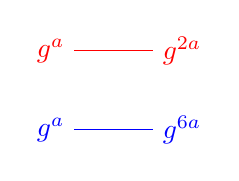
\begin{tikzpicture}
        \uncover<2->{\draw[red] (0,0) node[anchor=east]{$g^a$} -- (1,0) node[anchor=west] {$g^{2a}$};}
        \uncover<3->{\draw[blue] (0,-1) node[anchor=east]{$g^a$} -- (1,-1) node[anchor=west] {$g^{6a}$};}
      \end{tikzpicture}

      \bigskip
      \begin{uncoverenv}<5->
        Automorphism group: \emph{$(\Z/13\Z)^\times$}.
      \end{uncoverenv}
    \end{column}
  \end{columns}
\end{frame}

%%

\begin{frame}
  \begin{block}{Group action}
    \emph{$\G\circlearrowright\E$}: A (finite) set $\E$ \emph{acted
      upon} by a group $\G$ \emph{freely} and \emph{transitively}:
    \begin{align*}
      * : \G × \E &→ \E\\
      \g * E &↦ E'
    \end{align*}
    \par\begin{description}
    \item[Compatibility:] \emph{$\g' * (\g * E) = (\g'\g)*E$} for all
      $\g,\g'\in\G$ and $E\in\E$;
    \item[Identity:] \emph{$\mathfrak{e} * E = E$} if and only if
      $\mathfrak{e}\in\G$ is the identity element;
    \item[Regularity:] for all $E,E'\in\E$ there exist a \emph{unique
        $\g\in\G$} such that \emph{$\g*E'=E$}.
      \setlength{\itemsep}{2em}
    \end{description}
  \end{block}
\end{frame}

%%

\begin{frame}{Cryptographic Group Actions \small(Alamati, D., Montgomery, Patranabis 2021)}
  \begin{block}{Hard Homogeneous Space (HHS) --- Couveignes 1997 \small(eprint:2006/291)}
    \emph{$\G\circlearrowright\E$} such that $\G$ is commutative and:
    \begin{itemize}
    \item \emph{Evaluating} $E' = \g*E$ is \emph{easy};
    \item \emph{Inverting} the action is \emph{hard}.
    \end{itemize}
  \end{block}

  \begin{block}{Example}
    Let $G$ be a group of order $13$, then \emph{$(\Z/13\Z)^\times \circlearrowright G$} defined by
    \[a * g := g^a\]
    is an HHS\dots\pause
    But
    \[\alert{g^a \cdot g^b = g^{a+b}}\]
    has no interpretation as a group action!
  \end{block}
\end{frame}

%%

\begin{frame}{Key exchange from group actions}
  \begin{description}
  \item[Public parameters:] A \emph{HHS $\G\circlearrowright \E$} of
    order $N$ (large, but not necessarily prime).
  \end{description}

  \bigskip
  
  \begin{center}
    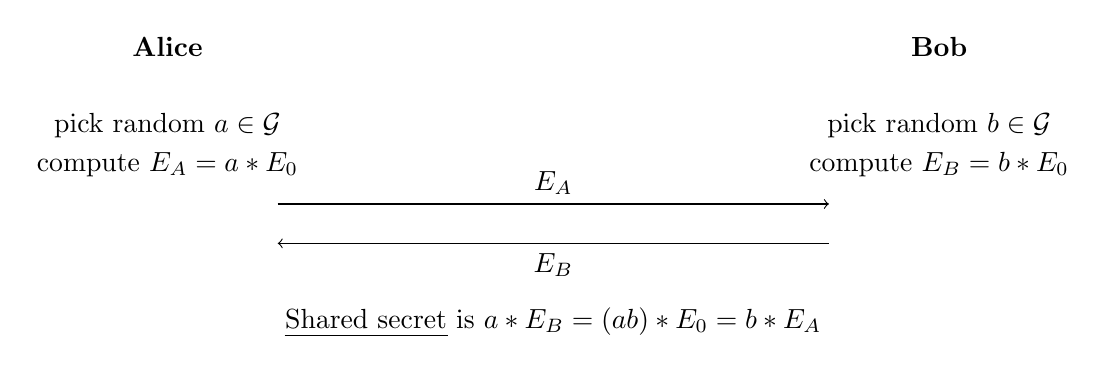
\begin{tikzpicture}[x=1.4cm]
      \node at (0,0) {\bf Alice};
      \node at (7,0) {\bf Bob};
      \node at (0,-1) {pick random \alert{$\a\in\G$}};
      \node at (0,-1.5) {compute $E_A=\a*E_0$};
      \node at (7,-1) {pick random \alert{$\b\in\G$}};
      \node at (7,-1.5) {compute $E_B=\b*E_0$};
      \draw[->]
      (1,-2) to node[auto] {$E_A$} (6,-2);
      \draw[->] (6,-2.5) to node[auto] {$E_B$} (1,-2.5);
      \node at (3.5,-3.5) {\emph{Shared secret} is \alert{$\a*E_B=(\a\b)*E_0=\b*E_A$}};
    \end{tikzpicture}
  \end{center}
\end{frame}

%%

\begin{frame}{Quantum security}

  \textbf{Fact:} Shor's algorithm \emph{does not apply} to Diffie-Hellman
  protocols from \emph{group actions}.

  \begin{block}{Subexponential attack\hfill\emph{$\exp(\sqrt{\log N\log\log N})$}}
    \begin{itemize}
    \item Reduction to the \emph{hidden shift problem} by evaluating
      the group action in \emph{quantum superposition} (subexponential
      cost);
    \item Well known reduction from the hidden shift to the
      \emph{dihedral (non-abelian) hidden subgroup problem};
    \item Kuperberg's algorithm solves the dHSP with a subexponential
      number of class group evaluations.
    \item Analyses suggest that $2^{64}$-qbit security may be achieved
      somewhere around $\log N \approx 2048$.
    \end{itemize}
  \end{block}
\end{frame}

%%

\begin{frame}{A $\Sigma$-protocol from group actions \small(Stolbunov 2008)}
  \begin{columns}
    \begin{column}{0.55\textwidth}
      Building block of Seasign and CSI-FiSh:

      \medskip
      \begin{itemize}
      \item<1-> A key pair \emph{$(\frak{s}, \frak{s}*E)$};
      \item<2-> Commit to a \emph{random element $\frak{r}*E$};
      \item<3-> Challenge with bit \emph{$b\in\{0,1\}$};
      \item<4-> Respond with \emph{$\frak{c} = \frak{r}/\frak{s}^b$};
      \item<5-> Verify that \emph{$\frak{c}*\frak{s^b}*E = \frak{r}*E$}.
      \end{itemize}

      \begin{block}{Zero-knowledge}<6->
        \centering
        Does not leak if:\\
        \alert{$\frak{c}$ is uniformly distributed} and independent from $\frak{s}$.
      \end{block}

    \end{column}  
    \begin{column}{0.40\textwidth}
      \centering
      \begin{tikzpicture}
        \node (g) at (0,0) {$E$};
        \node (gs) at (3,0) {$E_s$};
        \path[->] (g) edge node[auto]{$\frak{s}$} (gs);
        \uncover<2->{
          \node (gr) at (1.5,-3) {$E_r$};
          \path[->] (g) edge node[auto,swap]{$\frak{r}$} (gr);
        }
        \uncover<4->{
          \path[dashed,->] (gs) edge node[auto]{$\frak{r}/\frak{s}$} (gr);
        }
      \end{tikzpicture}
    \end{column}  
  \end{columns}
\end{frame}

%%

\begin{frame}{How isogenies may fail the axioms}
  \begin{block}{\alt<2->{\sout{Hard Homogeneous Space (HHS)}}{Hard
        Homogeneous Space (HHS)} \uncover<2->{Restricted Effective Group Action (REGA)}}
    \emph{$\G\circlearrowright\E$} such that $\G$ is commutative and:
    \begin{itemize}
    \item \emph{Inverting} the action is \emph{hard}.
    \item \alt<2->{\sout{\emph{Evaluating} $E' = \g*E$ is \emph{easy};}}{\emph{Evaluating} $E' = \g*E$ is \emph{easy};}
    \item<2-> There is a small list of elements
      \emph{$(\g_1, \ldots, \g_n)$} such that evaluating $E' = \g_i*E$
      is easy.
    \end{itemize}
  \end{block}
  
  \begin{uncoverenv}<3->
    Assume that $(\g_1, \ldots, g_n)$ generates $\G$:
    \begin{align*}
      \Z^n &\twoheadrightarrow \G\\
      (a_1,\ldots,a_n)&\mapsto \g_1^{a_1}\cdots g_n^{a_n}
    \end{align*}
    Extend $\G\circlearrowright\E$ to an action
    \emph{$\Z^n\circlearrowright\E$} (not free):
    \[(a_1, \ldots, a_n) * E \quad:=\quad \g_1^{a_1} * \cdots * \g_n^{a_n} * E.\]
  \end{uncoverenv}
\end{frame}

%%

\begin{frame}{Crypto from REGAs}
  \[(a_1, \ldots, a_n) * E \quad:=\quad \g_1^{a_1} * \cdots * \g_n^{a_n} * E.\]

  \begin{itemize}
  \item Evaluation efficient for vectors in $\Z^n$ of \emph{small norm};
  \item Key exchange works unmodified;
  \item<2-> Signature breaks down:
    \begin{columns}
      \begin{column}{0.40\textwidth}
        \begin{itemize}
        \item A key pair \emph{$(\vec{s}, \vec{s}*E)$};
        \item Commit to a \emph{random element $\vec{r}*E$};
        \item Challenge with bit \emph{$b\in\{0,1\}$};
        \item \alert{Respond with $\vec{c} = \vec{r} - b\cdot\vec{s}$};
        \item Verify that \emph{$\vec{c}*(b\cdot\vec{s})*E = \vec{r}*E$}.
        \end{itemize}
        Distribution of \alert{$\vec{r}-\vec{s}$} depends on \alert{$\vec{s}$}.
      \end{column}
      \begin{column}{0.40\textwidth}
        \centering
        \begin{tikzpicture}
          \node (g) at (0,0) {$E$};
          \node (gs) at (3,0) {$E_s$};
          \path[->] (g) edge node[auto]{$\vec{s}$} (gs);
          \node (gr) at (1.5,-3) {$E_r$};
          \path[->] (g) edge node[auto,swap]{$\vec{r}$} (gr);
          \path[dashed,->] (gs) edge node[auto]{$\vec{r} - \vec{s}$} (gr);
        \end{tikzpicture}
      \end{column}
    \end{columns}

    \medskip
    Fix: \emph{rejection sampling}. Very expensive!
  \end{itemize}
\end{frame}

%%

\begin{frame}{How to transform a REGA in an Effective Group Action again}
  \begin{align*}
    \Z^n &\twoheadrightarrow \G\\
    (a_1,\ldots,a_n)&\mapsto \g_1^{a_1}\cdots g_n^{a_n}
  \end{align*}
  The kernel is an integral lattice $\Lambda$, and
  \emph{$\G \simeq Z^n/\Lambda$}.

  \begin{enumerate}
  \item Compute the kernel $\Lambda$
    \begin{itemize}
    \item In \emph{subexponential} $L(1/2)$ time for isogenies, or
    \item In \emph{quantum polynomial time} for any group;
    \end{itemize}
  \item Compute generators of $\Z^n/\Lambda$;
  \item Use lattice reduction to convert elements of $\Z^n/\Lambda$ to
    vectors of \emph{small norm}.
  \end{enumerate}

  \pause
  \begin{block}{Applications \small(Beullens, Kleinjung, Vercauteren 2019; D., Meyer 2020)}
    \begin{itemize}
    \item \emph{CSI-FiSh}: reasonably short and not too slow signatures.
    \item If \emph{$\G=\langle\g\rangle$} is cyclic of order
      \emph{$N$}, explicit action \emph{$\Z/N\Z\circlearrowright\E$}:
      $\qquad a * E := \g^a * E$\\
      $\to$ \emph{threshold signatures} via Shamir secret sharing.
    \end{itemize}
  \end{block}
\end{frame}

%%

\begin{frame}[plain]
  \begin{beamercolorbox}[sep=0.1px,center,wd=\paperwidth,sep=0.5\paperheight]{palette tertiary}
    \Huge\centering Something new
  \end{beamercolorbox}
\end{frame}

%%

\begin{frame}{Objects \uncover<2>{and Morphisms}}
  \centering
  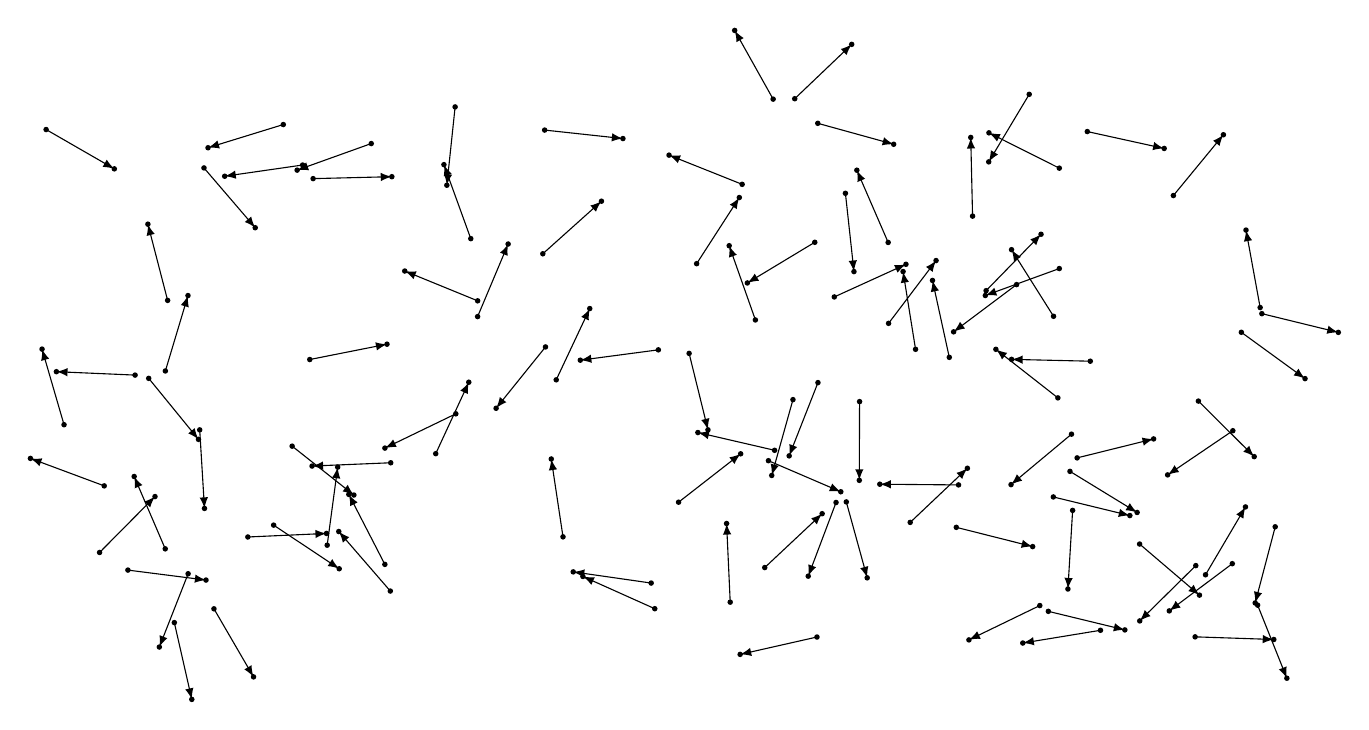
\begin{tikzpicture}
    \pgfmathsetseed{12345}
    \foreach \i in {1,...,100} {
      \pgfmathparse{16*random()}
      \let\x\pgfmathresult
      \pgfmathparse{7*random()}
      \let\y\pgfmathresult
      \pgfmathparse{360*random()}
      \let\ang\pgfmathresult
      \pgfmathparse{7*random()}
      \fill (\x,\y) circle (1pt) +(\ang:1) circle (1pt);
      \uncover<2>{\draw[-latex] (\x,\y) to +(\ang:1);}
    }
  \end{tikzpicture}  
\end{frame}

%%

\begin{frame}{More than graphs\dots}
  \begin{itemize}
  \item A finite set of \emph{objects} $\E$,
  \item For each pair $A,B\in\E$ a set of \emph{morphisms} $\Hom(A,B)$
  \end{itemize}

  \vfill
  
  \centering
  \begin{tikzpicture}
    \node (E1) at (0,0) {$B$};
    \node (E) at (6,0) {$A$};

    \draw[-latex] (E) edge node[above] {$φ$} (E1);
    \node at (3,-1.5) {$φ ∈ \Hom(A,B)$};

    \uncover<2->{
      \draw[-latex] (E) edge[loop,out=45,in=-45,looseness=10] node[right] {$ω$} (E);
      \node at (8,-1.5) {$ω ∈ \Hom(A,A)$};
    }
  \end{tikzpicture}
\end{frame}

%%

\begin{frame}{Transitively closed}
  \centering
  \begin{tikzpicture}
    \node (A) at (0,0) {$A$};
    \node (B) at (-6,0) {$B$};
    \node (C) at (-12,0) {$C$};

    \draw[-latex]
    (A) edge node[above] {$φ$} (B)
    (B) edge node[above] {$ψ$} (C);

    \uncover<2->{
      \draw[-latex]
      (A) edge[bend left] node[below] {$ψ∘φ$} (C);
    }
  \end{tikzpicture}
\end{frame}

%%

\begin{frame}{Identity morphisms}
  \centering
  \begin{tikzpicture}
    \node (A) at (0,0) {$A$};
    \node (B) at (-6,0) {$B$};
    \draw[-latex]
    (A) edge node[above] {$φ$} (B)
    (A) edge[loop,out=45,in=-45,looseness=10] node[right] {$1_A$} (A)
    (B) edge[loop,out=135,in=225,looseness=10] node[left] {$1_B$} (B);
    \node at (-3,-1.5) {$1_A∘φ \;=\; φ \;=\; φ∘1_B$};
  \end{tikzpicture}
\end{frame}

%% 

\begin{frame}{Ab-categories}
  \large
  \begin{itemize}
    \setlength{\itemsep}{2em}
  \item $\Hom(A,B)$ is a group
  \item Distributivity:
    \begin{align*}
      φ∘(ψ+χ) &= (φ∘ψ)+(φ∘χ)\\[2em]
      (ψ+χ)∘φ &= (ψ∘φ)+(χ∘φ)\\
    \end{align*}
  \item It follows that \emph{$\End(A) := \Hom(A,A)$} is a ring.
  \end{itemize}
\end{frame}

%%

\begin{frame}{Computational properties}
  \large
  \begin{itemize}
    \setlength{\itemsep}{2em}
  \item Every object and every morphism has a unique representation as
    a string;
  \item The representation of a morphism $\phi:A\to B$ identifies $A$
    and $B$;
  \item There exists efficient algorithms to verify that a string
    represents an object/morphism;
  \item There exists an \emph{origin object} $O \in \E$ whose
    representation is known;
  \item \dots
  \end{itemize}
\end{frame}

%%

\begin{frame}{\textit{Walking}}
  \large
  Efficient algorithm for:
  
  \bigskip
  \begin{description}
  \item[Input:] Object $A$
  \item[Output:]
    \begin{itemize}
    \item Uniformly random object $B$,
    \item Random morphism $\phi:A\to B$.
    \end{itemize}
  \end{description}
\end{frame}

%%

\begin{frame}{\textit{Triangulating}}
  \centering
  \begin{tikzpicture}
    \node (O) at (0,0) {$O$};
    \node (A) at (2,-4) {$A$};
    \node (B) at (-2,-4) {$B$};
    \draw[-latex] (O) edge (A) edge (B);
    \node at (0,-5) {\emph{Input}};
    \uncover<2->{
      \node (AA) at (10,-4) {$A$};
      \node (BB) at (6,-4) {$B$};
      \draw[-latex] (AA) edge node[above] {random} (BB);
      \node at (8,-5) {\emph{Output}};
    }
  \end{tikzpicture}
\end{frame}

%%

\begin{frame}{Assumption 1}
  Given $A, B$ hard to find $\phi: A \to B$

  \vfill
  
  \centering
  \begin{tikzpicture}
    \node (A) at (0,0) {$A$};
    \node (B) at (-6,0) {$B$};
    \draw[-latex,dashed] (A) edge (B);
  \end{tikzpicture}
\end{frame}

%%

\begin{frame}{Assumption 2}
  These two distributions are indistinguishable:

  \vfill

  \begin{columns}
    \begin{column}{0.5\textwidth}
      \begin{itemize}
      \item Given $A$,
      \item \emph{\textit{Walk} $\phi : A \to B$,}
      \end{itemize}
    \end{column}
    \begin{column}{0.5\textwidth}
      \begin{itemize}
      \item Given $O \to A$,
      \item Sample random $O \to B$,
      \item \emph{\textit{Triangulate} $\phi : A \to B$} 
      \end{itemize}
    \end{column}
  \end{columns}
\end{frame}

%%

\begin{frame}{Signatures}
  \large
  \centering
  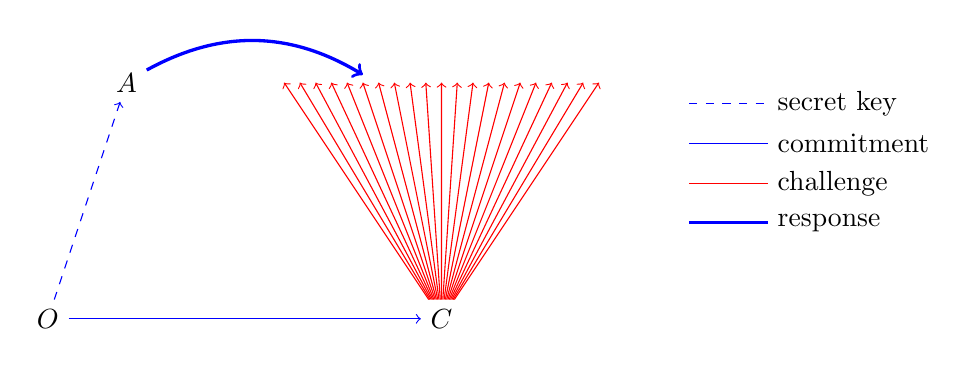
\begin{tikzpicture}
    \node (E0) at (1,3) {$A$};
    \node (EA) at (0,0) {$O$};
    \draw [blue,dashed,<-] (E0) edge (EA);

    \uncover<2->{
      \node (Ec) at (5,0) {$C$};
      \draw [blue] [->] (EA) to (Ec);
    }

    \uncover<3->{
      \foreach \x in {3,3.2,...,7} {
        \draw [red,->] (Ec) -- (\x,3);
      }
    }
    
    \uncover<4->{
      \draw [blue,very thick,->] (E0) to[bend left] (4,3.1);
    }
    
    \matrix [right] at (8,2) {
      \draw[dashed] (0,0) edge[blue] (1,0) (1,0) node {secret key};\\
      \uncover<2->{\draw (0,0) edge[blue] (1,0) (1,0) node {commitment};}\\
      \uncover<3->{\draw (0,0) edge[red] (1,0) (1,0) node {challenge};}\\
      \uncover<4->{\draw (0,0) edge[blue,very thick] (1,0) (1,0) node {response};}\\
    };
  \end{tikzpicture}
\end{frame}

%%

\begin{frame}[plain]
  \centering
  \begin{tikzpicture}[remember picture,overlay]
    \begin{scope}[xscale=1.7,yshift=-15,opacity=0.8]
      \def\crater{12}
      \def\jumpa{-8}
      \def\jumpb{9}
      \def\diam{5cm}

      \foreach \i in {1,...,\crater} {
        \draw[blue] (360/\crater*\i : \diam) to[bend right] (360/\crater*\i+360/\crater : \diam);
        \draw[red] (360/\crater*\i : \diam) to[bend right] (360/\crater*\i+\jumpa*360/\crater : \diam);
        \draw[green] (360/\crater*\i : \diam) to[bend right=50] (360/\crater*\i+\jumpb*360/\crater : \diam);
      }
    \end{scope}
    
    \draw (0,0.5) node{\Huge\bf Thank you};
    \draw (0,-0.6) node{\large\url{https://defeo.lu/}};
    \draw (0,-1.3) node{\large\includegraphics[height=0.9em]{mastodon.png}~\href{https://twitter.com/luca_defeo}{@luca\_defeo@ioc.exchange}};
    \draw (0,-1.9) node{\large
\includegraphics[height=0.9em]{twitter.png}~\href{https://twitter.com/luca_defeo}{@luca\_defeo}};
  \end{tikzpicture}
\end{frame}

%%

\end{document}


% LocalWords:  Isogeny abelian isogenies hyperelliptic supersingular Frobenius
% LocalWords:  isogenous
